\documentclass{article}\usepackage[]{graphicx}\usepackage[]{color}
%% maxwidth is the original width if it is less than linewidth
%% otherwise use linewidth (to make sure the graphics do not exceed the margin)
\makeatletter
\def\maxwidth{ %
  \ifdim\Gin@nat@width>\linewidth
    \linewidth
  \else
    \Gin@nat@width
  \fi
}
\makeatother

\definecolor{fgcolor}{rgb}{0.345, 0.345, 0.345}
\newcommand{\hlnum}[1]{\textcolor[rgb]{0.686,0.059,0.569}{#1}}%
\newcommand{\hlstr}[1]{\textcolor[rgb]{0.192,0.494,0.8}{#1}}%
\newcommand{\hlcom}[1]{\textcolor[rgb]{0.678,0.584,0.686}{\textit{#1}}}%
\newcommand{\hlopt}[1]{\textcolor[rgb]{0,0,0}{#1}}%
\newcommand{\hlstd}[1]{\textcolor[rgb]{0.345,0.345,0.345}{#1}}%
\newcommand{\hlkwa}[1]{\textcolor[rgb]{0.161,0.373,0.58}{\textbf{#1}}}%
\newcommand{\hlkwb}[1]{\textcolor[rgb]{0.69,0.353,0.396}{#1}}%
\newcommand{\hlkwc}[1]{\textcolor[rgb]{0.333,0.667,0.333}{#1}}%
\newcommand{\hlkwd}[1]{\textcolor[rgb]{0.737,0.353,0.396}{\textbf{#1}}}%

\usepackage{framed}
\makeatletter
\newenvironment{kframe}{%
 \def\at@end@of@kframe{}%
 \ifinner\ifhmode%
  \def\at@end@of@kframe{\end{minipage}}%
  \begin{minipage}{\columnwidth}%
 \fi\fi%
 \def\FrameCommand##1{\hskip\@totalleftmargin \hskip-\fboxsep
 \colorbox{shadecolor}{##1}\hskip-\fboxsep
     % There is no \\@totalrightmargin, so:
     \hskip-\linewidth \hskip-\@totalleftmargin \hskip\columnwidth}%
 \MakeFramed {\advance\hsize-\width
   \@totalleftmargin\z@ \linewidth\hsize
   \@setminipage}}%
 {\par\unskip\endMakeFramed%
 \at@end@of@kframe}
\makeatother

\definecolor{shadecolor}{rgb}{.97, .97, .97}
\definecolor{messagecolor}{rgb}{0, 0, 0}
\definecolor{warningcolor}{rgb}{1, 0, 1}
\definecolor{errorcolor}{rgb}{1, 0, 0}
\newenvironment{knitrout}{}{} % an empty environment to be redefined in TeX

\usepackage{alltt}

\usepackage{fancyhdr}
\usepackage{amsmath}
\usepackage{amssymb}
\usepackage{xparse}
\usepackage{bbm}
\usepackage[margin=1in]{geometry}
\pagestyle{fancy}
\lhead{isg2}

\newcommand{\argmin}{\operatornamewithlimits{argmin}}
\IfFileExists{upquote.sty}{\usepackage{upquote}}{}
\begin{document}

\begin{center}
{\bf {\Large STAT 365 Final Project: Analysis of Online Pizza Altruism}}\\


\vspace{3mm}

{\bf Ian Gonzalez}
\end{center}



% Current problems:
% 1. No way to incorporate the LDA analysis I did.
% 2. The test data is in a different format and difficult to test on
% (requires kaggle submission)


% SOLUTIONS (YAY): 
% 1. Make some plots indicating the overlap between my sets and the 
% given sets. Describe some words that I added from my analysis. Add
% topic model for adjectives, see if anything interesting comes up.
% describe the result of this.

% Also, remember to make plots of how often words from each topic
% come up across the data!

% 2. Simply remove part of the given training set and use it as a test
% set.



\section{Introduction}

\subsection{Topic overview}

The online community reddit.com, one of the top 100 sites in the world, is a public forum composed of numerous subcommunities called subreddits. Many aspects of the site focus on user altruism -- for example, users can buy each other ``reddit gold" as a reward for good comments or posts. One of the earliest and most prominent subcommunities devoted to inter-Redditor altruism is Random Acts of Pizza, a subreddit where users can make posts requesting pizza deliveries to their physical locations.

Given the high amount of traffic on reddit and the well-documented nature of the posts in RAOP, the subcommunity is a useful case study for examining what factors cause people to respond altruistically to requests. At the very least, the data from this community may be able to shed some light on how people give over the internet, when standard social factors such as face-to-face interaction are eliminated. We might expect to find a subset of features that are highly predictive of whether or not a user's request is successful (i.e. results in them receiving a pizza).

\subsection{Existing work}

A recent paper [1] published a dataset consisting of data from a few thousand posts on RAOP. The data set consists of features such as the text of the request, the text of request title, the timestamp of the post, the user's ``karma" (a measure of community standing), and the number of upvotes and downvotes the post received. One of the difficulties of training a predictor on this data set is the conversion of the qualitative data in the request text and title into some quantitative measures.

The paper also produced an analysis of the dataset -- the authors created a logistic regression model to predict the user's success. In order to extract quantitative data from the seemingly qualitative post text, they used topic modeling to identify five distinct narratives in the data, which were then quantified via word count features of words that correlate strongly with those narratives. The presence of these narratives seemed to be highly predictive of post success in the final model. They also analyzed the politeness and temporality of the posts, although neither analysis produced highly predictive features.

\subsection{Goals}

The goal of this project is to verify and expand upon the analysis done in the paper. I will examine and visualize the data more thoroughly than done in the paper, and I will try other linguistic analysis methods on the textual data. Ultimately, I will also try other learning methods beyond logistic regression for learning the data without overfitting.

The topic modeling done on the posts seems like a good place to experiment, since making the topic word clusters more precise can only improve the model (assuming that good differentiation between topics is predictive). I will try a different topic model based on latent Dirichlet allocation and compare its success with the topics generated in the paper. I may also experiment with topic modeling on the adjectives in the posts, since they may give more insight into the tone of the post.

I will also try to focus on adding some features that were not focused on in the paper. I expect that spelling and grammar mistakes will reduce the chances of success for the poster.

As for predictive modeling, I will attempt to improve upon the performance of the classifier using feature normalization and by experimenting with an adaboost-trained learner.


%%%%%%%%%%%%%%%%%%%%%%%%%%%%%%%%%%%%%%%%%%%%%%%%%%%%%%%%%%%%%%%%%
\newpage


\section{Data cleaning and feature extraction}

The dataset came in a JSON format, which was converted into a more R-friendly dataframe. Relatively meaningless features such as request ids, timestamps, and usernames were then stripped from the data, and a feature accounting for the length of the request was added. Most of the following analysis was then done on the request text and title, which needed more processing.

The R package openNLP was used to create sentence and word annotations for the posts, which were then used to label the part of speech for every word in the posts.

\begin{knitrout}
\definecolor{shadecolor}{rgb}{0.969, 0.969, 0.969}\color{fgcolor}\begin{kframe}
\begin{alltt}
  \hlstd{sent_annotator} \hlkwb{<-} \hlkwd{Maxent_Sent_Token_Annotator}\hlstd{()}
  \hlstd{word_annotator} \hlkwb{<-} \hlkwd{Maxent_Word_Token_Annotator}\hlstd{()}
  \hlstd{reqtext} \hlkwb{<-} \hlkwd{sapply}\hlstd{(reqtext, as.String)}

  \hlcom{# do word and sentence annotation:}
  \hlstd{annotations} \hlkwb{<-} \hlkwd{lapply}\hlstd{(reqtext,} \hlkwa{function}\hlstd{(}\hlkwc{req}\hlstd{) \{}
    \hlkwa{if} \hlstd{(req} \hlopt{==} \hlstr{""}\hlstd{) \{}\hlkwd{list}\hlstd{()\}}
    \hlkwa{else} \hlstd{\{}\hlkwd{annotate}\hlstd{(req,} \hlkwd{list}\hlstd{(sent_annotator, word_annotator))\}}
  \hlstd{\})}

  \hlcom{#do pos annotation:}
  \hlstd{pos_annotator} \hlkwb{<-} \hlkwd{Maxent_POS_Tag_Annotator}\hlstd{()}
  \hlstd{pos_annots} \hlkwb{<-} \hlkwd{lapply}\hlstd{(}\hlnum{1}\hlopt{:}\hlkwd{length}\hlstd{(reqtext),} \hlkwa{function}\hlstd{(}\hlkwc{i}\hlstd{) \{}
    \hlkwa{if} \hlstd{(reqtext[i]} \hlopt{==} \hlstr{""}\hlstd{) \{}\hlkwd{list}\hlstd{()\}}
    \hlkwa{else} \hlstd{\{}\hlkwd{annotate}\hlstd{(reqtext[i], pos_annotator, annotations[[i]])\}}
  \hlstd{\})}
\end{alltt}
\end{kframe}
\end{knitrout}

This information was then used to extract only the nouns from the posts. The nouns, which were used for feature creation in the paper as well, should generally adhere fairly closely to the topics of the posts, although the adjectives and verbs likely merit more exploration.

\begin{knitrout}
\definecolor{shadecolor}{rgb}{0.969, 0.969, 0.969}\color{fgcolor}\begin{kframe}
\begin{alltt}
\hlstd{nouns} \hlkwb{<-} \hlkwd{lapply}\hlstd{(}\hlnum{1}\hlopt{:}\hlkwd{length}\hlstd{(reqtext),} \hlkwa{function}\hlstd{(}\hlkwc{i}\hlstd{)\{}
  \hlkwa{if} \hlstd{(reqtext[i]} \hlopt{==} \hlstr{""}\hlstd{) \{}\hlkwd{character}\hlstd{(}\hlnum{0}\hlstd{)\}}
  \hlkwa{else} \hlstd{\{}
    \hlstd{wordanns} \hlkwb{<-} \hlkwd{subset}\hlstd{(pos_annots[[i]], type}\hlopt{==}\hlstr{"word"}\hlstd{)}
    \hlstd{words} \hlkwb{<-} \hlkwd{getwords}\hlstd{(reqtext[i], wordanns)}
    \hlstd{only_nouns} \hlkwb{<-} \hlkwd{as.character}\hlstd{(}\hlkwd{getpos}\hlstd{(words, wordanns,} \hlkwd{c}\hlstd{(}\hlstr{"NN"}\hlstd{,}\hlstr{"NNP"}\hlstd{,}\hlstr{"NNS"}\hlstd{)))}
  \hlstd{\}}
\hlstd{\})}
\end{alltt}
\end{kframe}
\end{knitrout}

The distribution of nouns in the posts could then be analyzed to reveal the underlying structure in the data.

\subsection{Clustering}

The paper claimed that using 5 underlying topics to group the posts was an effective model for predicting request success. This claim was tested by using unsupervised clustering on the posts and observing how many linguistic clusters seem to appear naturally in the data.

Each post was first converted into a bag-of-words vector encoding how many times the top 100 nouns appeared in the post. Principal component analysis was done on the resulting data to reduce its dimensionality to 2 (for less expensive clustering and visualization).

\begin{knitrout}
\definecolor{shadecolor}{rgb}{0.969, 0.969, 0.969}\color{fgcolor}\begin{kframe}
\begin{alltt}
\hlkwa{for} \hlstd{(i} \hlkwa{in} \hlnum{1}\hlopt{:}\hlkwd{length}\hlstd{(nouns)) \{}
  \hlstd{noun_bags[i,]} \hlkwb{<-} \hlkwd{sapply}\hlstd{(top_nouns,} \hlkwa{function}\hlstd{(}\hlkwc{nn}\hlstd{)\{}\hlkwd{sum}\hlstd{(nouns[[i]]} \hlopt{==} \hlstd{nn)\})}
\hlstd{\}}
\hlstd{noun_PCA} \hlkwb{<-} \hlkwd{prcomp}\hlstd{(noun_bags)}

\hlstd{noun_PC1} \hlkwb{<-} \hlstd{noun_PCA}\hlopt{$}\hlstd{rotation[,}\hlnum{1}\hlstd{]}
\hlstd{noun_PC2} \hlkwb{<-} \hlstd{noun_PCA}\hlopt{$}\hlstd{rotation[,}\hlnum{2}\hlstd{]}

\hlstd{noun_dim_reduce} \hlkwb{<-} \hlkwd{cbind}\hlstd{(noun_PC1, noun_PC2)}
\hlstd{noun_reduced} \hlkwb{<-} \hlkwd{t}\hlstd{(noun_dim_reduce)} \hlopt \hlkwd{t}\hlstd{(noun_bags)}
\end{alltt}
\end{kframe}
\end{knitrout}


These vectors were then plotted on the first 2 principal components of the data to produce the following visualization:

\begin{knitrout}
\definecolor{shadecolor}{rgb}{0.969, 0.969, 0.969}\color{fgcolor}

{\centering 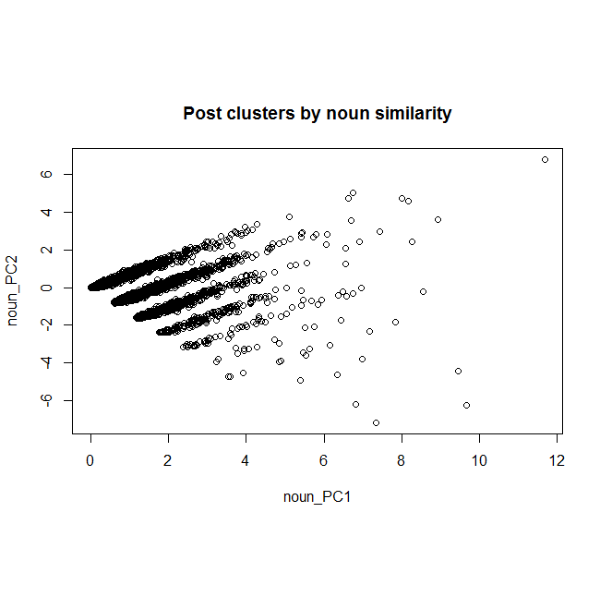
\includegraphics[width=\maxwidth]{figure/unnamed-chunk-5-1} 

}



\end{knitrout}

There appear to be 5 naturally separable clusters within the data, which confirms the assumption made in the paper about the number of distinct topics. To confirm this more formally, the R clValid cluster validation package was used to show that across all possible cluster counts from 3 to 10, 5 had the highest connectivity score (about 72.8).

\begin{knitrout}
\definecolor{shadecolor}{rgb}{0.969, 0.969, 0.969}\color{fgcolor}\begin{kframe}
\begin{alltt}
\hlstd{valid_nn_clust}\hlkwb{<-} \hlkwd{clValid}\hlstd{(}\hlkwd{t}\hlstd{(noun_reduced),} \hlnum{3}\hlopt{:}\hlnum{10}\hlstd{,}
                         \hlkwc{clMethods} \hlstd{=} \hlstr{"kmeans"}\hlstd{,}
                         \hlkwc{validation}\hlstd{=}\hlstr{"internal"}\hlstd{)}
\hlkwd{optimalScores}\hlstd{(valid_nn_clust)}
\end{alltt}
\end{kframe}
\end{knitrout}


\subsection{Topic modeling}

As mentioned in the introduction, one of the more interesting and challenging aspects of this dataset is transforming the words in the posts into meaningfully distinct numerical features. The NLP problem that this corresponds to is known as topic modeling -- the problem is to find a series of topics, which are essentially probability distributions over words in some vocabulary, that could have produced the words in a set of documents. These topics will, ideally, roughly correspond to words that relate to some general idea such as ``biology" or ``chemistry" [2]. Topics can be easily quantified with word count features that count the number of times words from a particular topic appear in a document.

\subsubsection{Latent Dirichlet Allocation (LDA)}

The previously published paper uses nonnegative matrix factorization (NMF) for topic modeling over the posts. A slightly simpler model is latent Dirichlet allocation (LDA). LDA assumes that the topics are distributions over some vocabulary, and that the given documents are generated by some random process that selects each word from one of the topics. It also assumes that there are some hidden parameters indicating what proportion of each document corresponds to each topic.

More formally, if we take the topics (vocab distributions) to be $\beta_1...\beta_K$, the topic proportions for document d to be $\theta_d$, the topic assignments for each word in document d to be $z_d[1]...z_d[n]$, and the words in document d to be $w_d[1]...w_d[n]$, then the joint distribution over the variables is 

\vspace{3mm}

$\prod\limits_{i=1}^K p(\beta_i) \prod\limits_{d=1}^D p(\theta_d)\left(\prod_{n=1}^N p(z_d[n]|\theta_d) p(w_d[n]|\beta, z_d[n])\right)$

\vspace{3mm}


The posterior distribution for this can then be approximated using a variety of algorithms [2]. More complete information about LDA can be found in cited paper 2.

An R implementation of LDA that uses Gibbs sampling was used in this project for topic modeling and the results of this analysis was compared to the results from the paper. In order to simplify the model and remove useless words, LDA was trained on only the top 100 nouns in this project.

\begin{knitrout}
\definecolor{shadecolor}{rgb}{0.969, 0.969, 0.969}\color{fgcolor}\begin{kframe}
\begin{alltt}
\hlstd{topmodel} \hlkwb{<-} \hlkwd{lda.collapsed.gibbs.sampler}\hlstd{(docfeats,}
                                        \hlkwc{K}\hlstd{=}\hlnum{5}\hlstd{,}
                                        \hlkwc{num.iterations} \hlstd{=} \hlnum{25}\hlstd{,}
                                        \hlkwc{vocab}\hlstd{=top_nouns,}
                                        \hlkwc{alpha}\hlstd{=}\hlnum{0.1}\hlstd{,} \hlkwc{eta}\hlstd{=}\hlnum{0.1}\hlstd{)}
\hlstd{topwords} \hlkwb{<-} \hlkwd{top.topic.words}\hlstd{(topmodel}\hlopt{$}\hlstd{topics,} \hlnum{10}\hlstd{,} \hlkwc{by.score}\hlstd{=T)}
\end{alltt}
\end{kframe}
\end{knitrout}

Numerical features for each topic were then created via simple word counts for each topic within each post:

\begin{knitrout}
\definecolor{shadecolor}{rgb}{0.969, 0.969, 0.969}\color{fgcolor}\begin{kframe}
\begin{alltt}
\hlstd{mywordcnt} \hlkwb{<-} \hlkwd{matrix}\hlstd{(}\hlnum{0}\hlstd{,} \hlkwc{nrow}\hlstd{=}\hlkwd{length}\hlstd{(reqtext),} \hlkwc{ncol}\hlstd{=K)}
\hlkwa{for} \hlstd{(i} \hlkwa{in} \hlnum{1}\hlopt{:}\hlstd{K) \{}
  \hlstd{mywordcnt[,i]} \hlkwb{<-} \hlkwd{sapply}\hlstd{(nouns,} \hlkwa{function}\hlstd{(}\hlkwc{nns}\hlstd{)\{}
    \hlkwd{sum}\hlstd{(nns} \hlopt \hlstd{topwords[,i])}
  \hlstd{\})}
\hlstd{\}}
\end{alltt}
\end{kframe}
\end{knitrout}

The words from the topics used in the paper were then used to create a separate word count feature matrix with an analogous method. This allowed for comparison of the results from my LDA approach and the NMF approach.

\subsection{Additional features}

Beyond the topic analysis, a few extra features were calculated for addition to the model. A binary variable was added to indicate whether or not the post contained an image link, which was determined with a simple regex. This feature captures the evidentiality characteristic of successful requests for altruistic behavior discussed in the paper.

Two additional features were added that attempted to capture how many errors were made in the post text and title. The rationale behind adding these features is that users are less likely to respond positively to requesters who sound uneducated or careless (since this seems to genrally be the case). Error count is a reasonable measure of how uneducated or careless a post sounds. The paper published on this data does not consider this factor in their model.

Using an R spell checker in the package qdap, the number of spelling errors in the title and the text of each post was counted. These counts were then normalized by the word length of their respective texts.

\begin{knitrout}
\definecolor{shadecolor}{rgb}{0.969, 0.969, 0.969}\color{fgcolor}\begin{kframe}
\begin{alltt}
\hlcom{# check for spelling errors}
\hlkwd{require}\hlstd{(qdap)}
\hlstd{has_errs} \hlkwb{<-} \hlkwd{sapply}\hlstd{(}\hlnum{1}\hlopt{:}\hlkwd{length}\hlstd{(jsonframe}\hlopt{$}\hlstd{request_title),} \hlkwa{function}\hlstd{(}\hlkwc{i}\hlstd{)\{}
  \hlkwd{length}\hlstd{(}\hlkwd{which_misspelled}\hlstd{(reqtext[i]))}\hlopt{/}\hlstd{(}\hlkwd{length}\hlstd{(reqwords[[i]])} \hlopt{+} \hlnum{1}\hlstd{)}
\hlstd{\})}
\hlstd{featframe}\hlopt{$}\hlstd{has_errs} \hlkwb{<-} \hlstd{has_errs}
\end{alltt}
\end{kframe}
\end{knitrout}

Finally, the other numeric features (upvotes and downvotes, karma, etc.) were combined with the linguistic features to make 2 separate data frames -- one with the topic features from my LDA analysis, and one with the topic features from the papers.

Both feature frames were then mean normalized, meaning that every data point was converted to a number of standard deviations from the mean.

\begin{knitrout}
\definecolor{shadecolor}{rgb}{0.969, 0.969, 0.969}\color{fgcolor}\begin{kframe}
\begin{alltt}
\hlstd{normalize} \hlkwb{<-} \hlkwa{function}\hlstd{(}\hlkwc{data}\hlstd{) \{(data} \hlopt{-} \hlkwd{mean}\hlstd{(data))}\hlopt{/}\hlkwd{sqrt}\hlstd{(}\hlkwd{var}\hlstd{(data))\}}
\end{alltt}
\end{kframe}
\end{knitrout}

\newpage

\section{Dataset visualization}

Principal component analysis was performed on the two datasets produced and both were projected onto the first 2 principal components for plotting purposes. Below we can see the results of plotting these datasets with green dots representing successful requests and red dots representing failed requests. 

The graphs show that the dataset using the topic features from the paper seems to get a bit more separation between the two classes than my features (the colors are not as mixed in the first plot).

\begin{knitrout}
\definecolor{shadecolor}{rgb}{0.969, 0.969, 0.969}\color{fgcolor}

{\centering 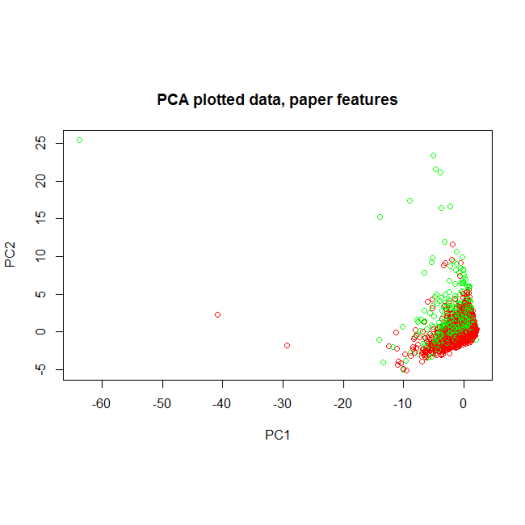
\includegraphics[width=\maxwidth]{figure/unnamed-chunk-11-1} 

}



\end{knitrout}


\begin{knitrout}
\definecolor{shadecolor}{rgb}{0.969, 0.969, 0.969}\color{fgcolor}

{\centering 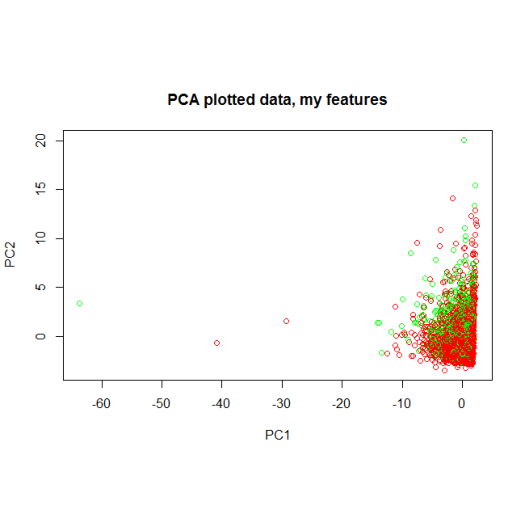
\includegraphics[width=\maxwidth]{figure/unnamed-chunk-12-1} 

}



\end{knitrout}


%%%%%%%%%%%%%%%%%%%%%%%%%%%%%%%%%%%%%%%%%%%%%%%%%%%%
\newpage

\section{Training models on the data}

The last step in the analysis was to use the two feature frames to train predictors. I tried a simple logistic regression model followed by an adaboosted learner using decision trees as the weak learners.

\subsection{Logistic regression}

First logistic regression was used to train a model on both datasets. The coefficients and corresponding p-values for the features added in the previous section can be seen below (most of the rest of the features were significant, and they did not vary between the models, so they are not included). The first set of coefficients is from the model trained with the features from the paper, and the second set is from the model trained with my features.

\begin{knitrout}
\definecolor{shadecolor}{rgb}{0.969, 0.969, 0.969}\color{fgcolor}\begin{kframe}
\begin{alltt}
\hlkwd{load}\hlstd{(}\hlstr{"glmcoeffs.rda"}\hlstd{)}
\end{alltt}


{\ttfamily\noindent\bfseries\color{errorcolor}{\#\# Error in readChar(con, 5L, useBytes = TRUE): cannot open the connection}}\begin{alltt}
\hlstd{sumglm4}\hlopt{$}\hlstd{coefficients[}\hlnum{22}\hlopt{:}\hlnum{30}\hlstd{,}\hlnum{3}\hlopt{:}\hlnum{4}\hlstd{]}
\end{alltt}


{\ttfamily\noindent\bfseries\color{errorcolor}{\#\# Error in eval(expr, envir, enclos): object 'sumglm4' not found}}\begin{alltt}
\hlstd{sumglm5}\hlopt{$}\hlstd{coefficients[}\hlnum{22}\hlopt{:}\hlnum{30}\hlstd{,}\hlnum{3}\hlopt{:}\hlnum{4}\hlstd{]}
\end{alltt}


{\ttfamily\noindent\bfseries\color{errorcolor}{\#\# Error in eval(expr, envir, enclos): object 'sumglm5' not found}}\end{kframe}
\end{knitrout}

Firstly, it is clear to see that the addition of the error features was meaningful; the low p-values and negative coefficients for the error feature in both the body and the title indicate that the presence of spelling errors in the post significantly decrease the posters chance of success.

Additionally, note that just as the paper on this dataset found, of the 5 narratives used 4 were beneficial and one was harmful to the requester's chance of success. One of the features (4) was also well above the 0.05 significance threshold, questioning its inclusion in the model (it's unclear why this happened -- there may be some discrepancy between my model and theirs that I haven't caught).

The model that used my features generated with LDA did slightly worse. Only 2 of the 5 topics were significant differentiators of successful and unsuccessful posts. This is likely due to overlap between the topic word lists and the fact that I didn't extend my word classes using a related word search like the paper did -- with a little more work, it seems like the LDA model may be able to do just as well.

Further supporting this idea is the fact that the training set accuracy for both classifiers was nearly identical (84\%). The test set accuracy was also close, with the first classifier beating out the one with my features by 0.5\% (83.5\%, 83.8\%).

\subsection{Adaboost}

Next, an adaboosted learner that used decision trees as weak learners was trained on both datasets.

Both models performed significantly better than the logistic regression models on the training sets. In fact, both boosted learners got 100\% accuracy on the training set. However, for the test sets the model using the paper features only showed an accuracy increase of about 1\%, and for the model using my features the accuracy actually remained constant. It seems that switching to adaboost actually only offers a slight performance increase for this prediction problem.

Below are the ROC curves for the two boosted learners. Clearly, the difference between their predictive power is not large. This is further supported by the fact that the AUC for the first model is 0.87, while the AUC for the second is 0.86.


\begin{knitrout}
\definecolor{shadecolor}{rgb}{0.969, 0.969, 0.969}\color{fgcolor}

{\centering 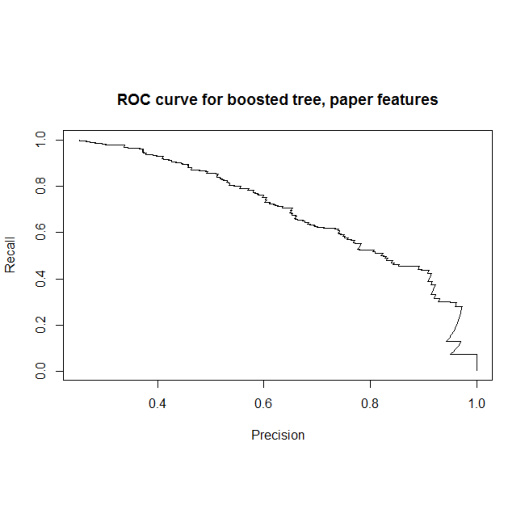
\includegraphics[width=\maxwidth]{figure/unnamed-chunk-14-1} 

}



\end{knitrout}

\begin{knitrout}
\definecolor{shadecolor}{rgb}{0.969, 0.969, 0.969}\color{fgcolor}

{\centering 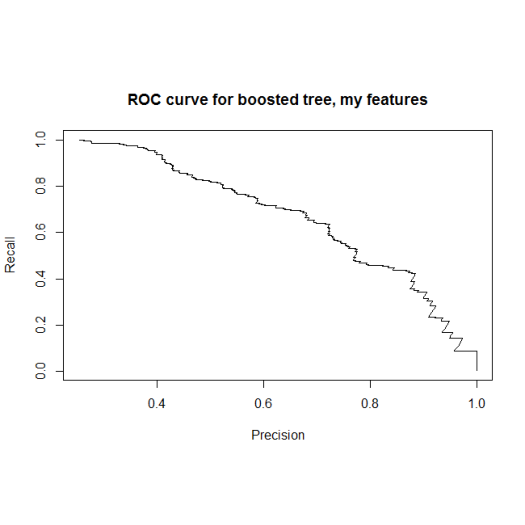
\includegraphics[width=\maxwidth]{figure/unnamed-chunk-15-1} 

}



\end{knitrout}

\section{Conclusions and future work}

It appears that using even a fairly naive LDA model with no addition of related words from wordbanks is enough to approach the predictive performance of the topic features used in the paper (which were generated with an NMF approach). With further expansion and removal of overlapping words, it may be possible to use the LDA model to define slightly more effective narrative lexicons for the 5 clusters that seem to be present in the data.

The addition of spelling error based features was a success. The features appeared to add significant differentiating power to the model, which follows the common-sense assumption that people are less likely to give free pizza to people that they perceive as careless or stupid.

Finally, the use of adaboost seems to be somewhat justified, since it did cause a slight performance boost in the more effective model. However, the modest increase may not be worth the additional computing time -- if the dataset is large, a simpler model like logistic regression is probably the right choice.

Additionally, although this was not mentioned above, feature normalization appeared to help predictive power immensely. The highest ROC AUC values in the paper were around 0.672. The predictors I trained did much better on the randomly selected test set. This may partially be because the test set I was using was much smaller than theirs, but it seems that feature normalization is the only significant change I made that could explain the rest of this improvement. It is also possible that the error features helped, but I doubt that this accounted for all of the change either.

Overall, the results of the paper were verified, and some possible avenues for minor expansions in effectiveness of prediction (adaboost and LDA) were identified. In future work in may be possible to obtain even higher accuracy by experimenting with other linguistic methods for analyzing the text. For example, an analysis of adjectives (which I didn't have time for) might reveal a lot about the tone of the posts.

\section{Data and Code}

The data used in this project can be found at https://www.kaggle.com/c/random-acts-of-pizza.

The R script used for the analysis will be made available on my GitHub page (https://github.com/iangonzalez), or is available upon request (I can be contacted at gonzalez.isv@gmail.com).

\section{References}

\hspace{4mm} 1. Tim Althoff, Cristian Danescu-Niculescu-Mizil, Dan Jurafsky. How to Ask for a Favor: A Case Study on the Success of Altruistic Requests, Proceedings of ICWSM, 2014.
 
\vspace{3mm}
 
2. Blei, David. Introduction to Probabilistic Topic Models. Communications of the ACM 2014. http://www.cs.princeton.edu/~blei/papers/Blei2011.pdf

\end{document}
